\begin{figure}
	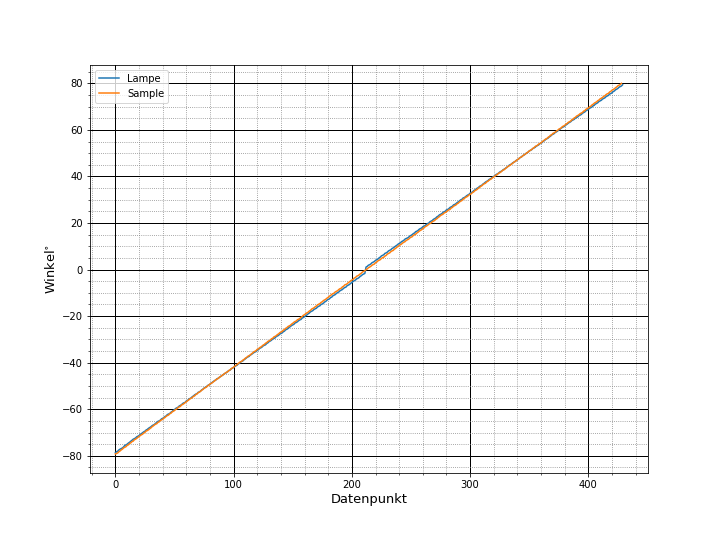
\includegraphics[scale=0.5]{Bilder/anhang/korrektur_channels_2}
	\centering
	\caption[Korrigierter Lampendatensatz 2. Silizium messung]{\small Auftragung der gemessenen Winkel für die Lampenmessung und erste Silizium Messung nach der Korrektur. Beide stimmen in den relevanten Bereichen bei ca. $30^{\circ}-40^{\circ}$ weitgehend überein.}
\end{figure}
\begin{figure}
	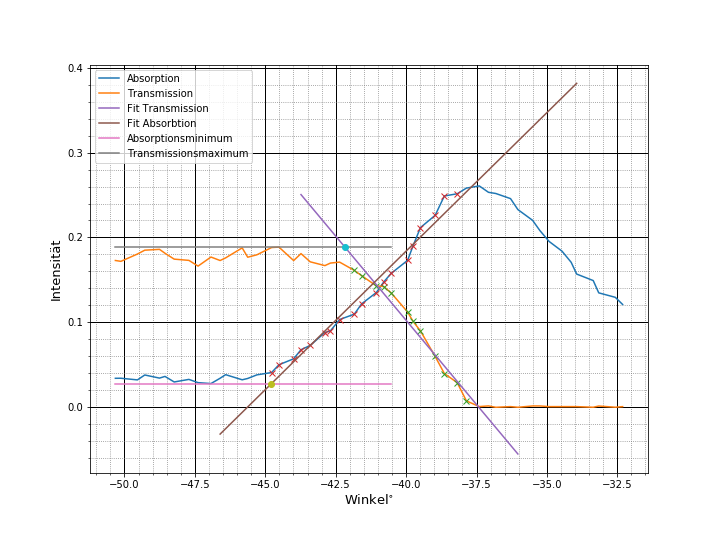
\includegraphics[scale=0.5]{Bilder/anhang/si_2_l}
	\centering
	\caption[Geraden Anpassungen 2. Silizium Messung links]{\small Auftragung von Intensität der normalisierten Datenreihen gegen die  Winkel in der Nähe der Stelle Gleichwahrscheinlicher Absorption und Transmission bei Winkeln kleiner als $0^\circ$. Es sind zusätzlich die angepassten Geraden zur Absorption und Transmission eingezeichnet. Die Horizontalen wurden durch die Maxima der dahinterliegenden Datenpunkte bestimmt. Die Schnittpunkte der Geraden mit ihren jeweiligen Horizontalen sind auch eingezeichnet.}
\end{figure}
\begin{figure}
	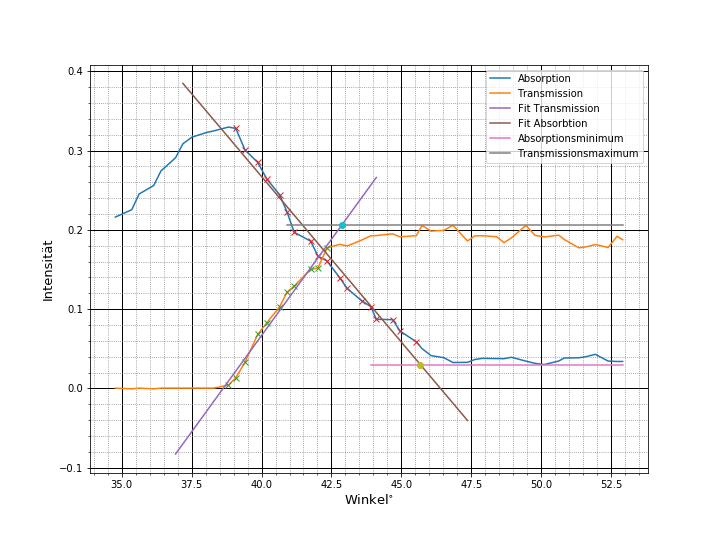
\includegraphics[scale=0.5]{Bilder/anhang/si_2_r}
	\centering
	\caption[Geraden Anpassungen 2. Silizium Messung rechts]{\small Auftragung von Intensität der normalisierten Datenreihen gegen die  Winkel der zweiten Silizium Messung in der Nähe der Stelle Gleichwahrscheinlicher Absorption und Transmission bei Winkeln größer als $0^\circ$. Es sind zusätzlich die angepassten Geraden zur Absorption und Transmission eingezeichnet. Die Horizontalen wurden durch die Maxima der dahinterliegenden Datenpunkte bestimmt. Die Schnittpunkte der Geraden mit ihren jeweiligen Horizontalen sind auch eingezeichnet.}
	\label{si_2_r}
\end{figure}
\begin{figure}
	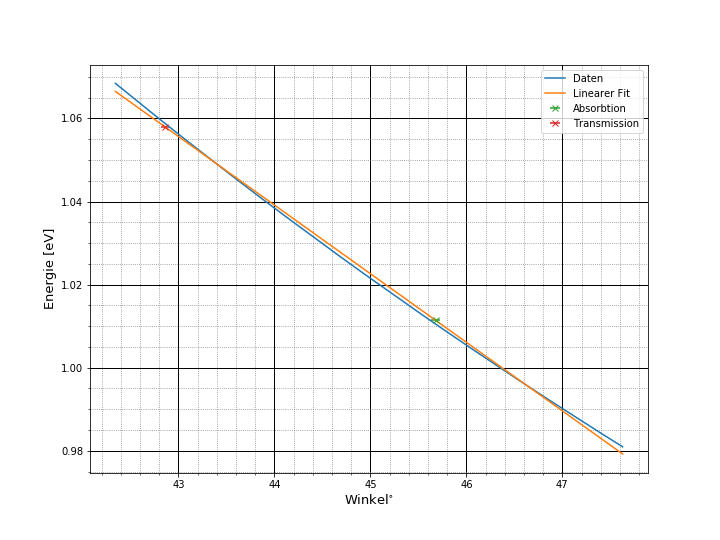
\includegraphics[scale=0.5]{Bilder/anhang/si_2_l_energie}
	\centering
	\caption[Energiebestimmung 2. Si Messung links]{\small Auftragung der Energie gegen den Winkel der zweiten Silizium Messung. Die angepasste Gerade und die beiden Schnittpunkte sind auch eingetragen.}
\end{figure}
\begin{figure}
	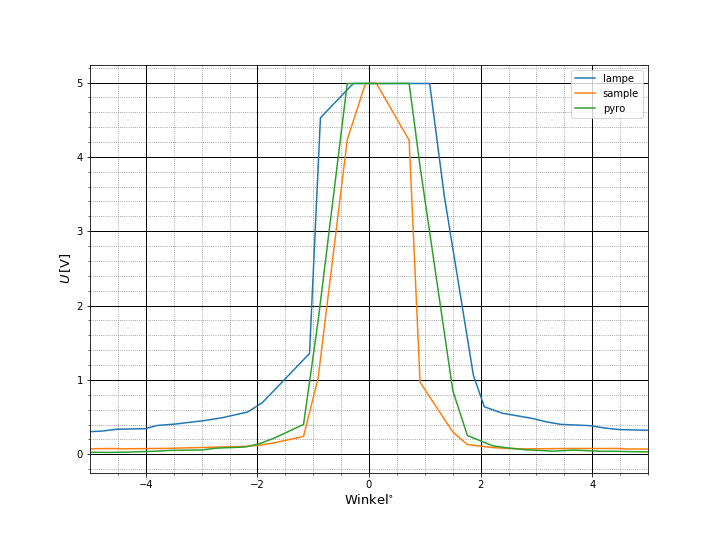
\includegraphics[scale=0.5]{Bilder/anhang/winkelkorrektur_vorher}
	\centering
	\caption[Mittelpunkt der 2. Si Messung vor Winkelkorrektur]{\small Auftragung der Intensität gegen den Winkel der zweiten Silizium Messung in der Nähe von $0^\circ$ vor der Korrektur.}
\end{figure}
\begin{figure}
	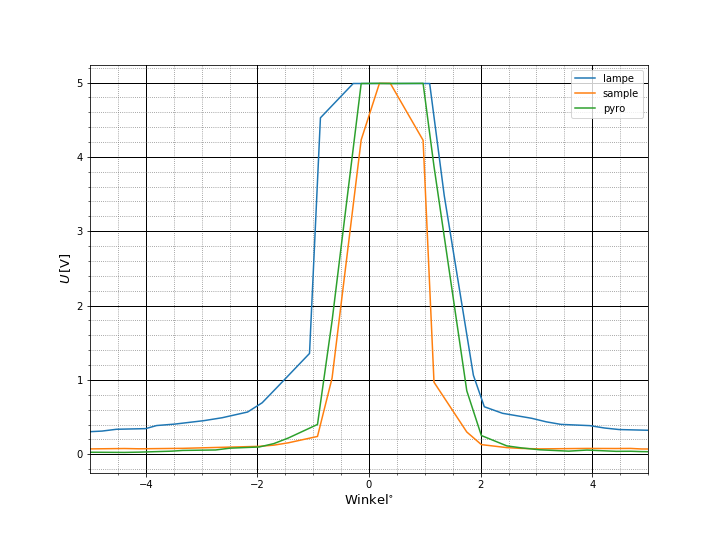
\includegraphics[scale=0.5]{Bilder/anhang/winkelkorrektur_nachher}
	\centering
	\caption[Mittelpunkt der 2. Si Messung vor Winkelkorrektur]{\small Auftragung der Intensität gegen den Winkel der zweiten Silizium Messung in der Nähe von $0^\circ$ nach der Korrektur.}
\end{figure}
\begin{figure}
	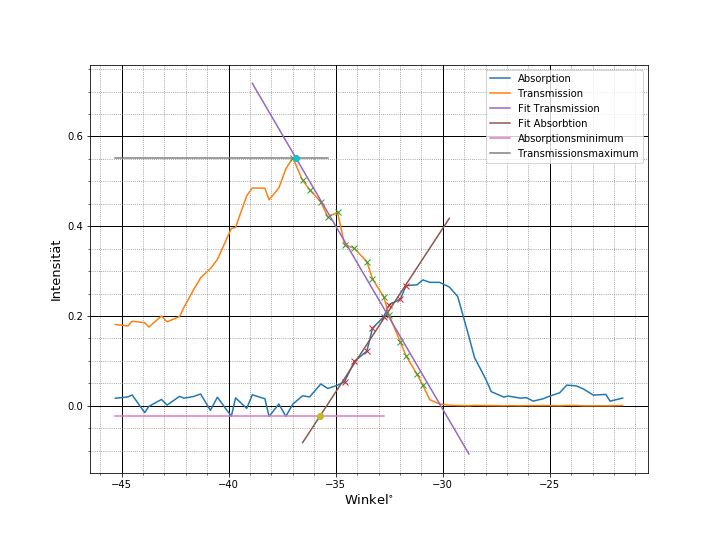
\includegraphics[scale=0.5]{Bilder/anhang/ge_r}
	\caption[Geraden Anpassungen Germanium Messung links]{\small Auftragung von Intensität der normalisierten Datenreihen von Germanium gegen die  Winkel in der Nähe der Stelle Gleichwahrscheinlicher Absorption und Transmission bei Winkeln größer als $0^\circ$. Es sind zusätzlich die angepassten Geraden zur Absorption und Transmission eingezeichnet. Die Horizontalen wurden durch die Maxima der dahinterliegenden Datenpunkte bestimmt. Die Schnittpunkte der Geraden mit ihren jeweiligen Horizontalen sind auch eingezeichnet.}
\end{figure}
\begin{figure}
	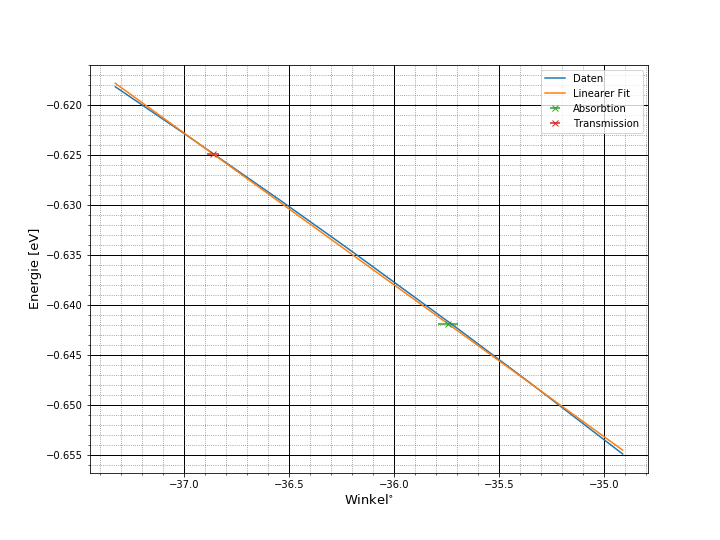
\includegraphics[scale=0.5]{Bilder/anhang/ge_l_energie}
	\centering
	\caption[Energiebestimmung Ge Messung links]{\small Auftragung der Energie gegen den Winkel der Germanium Messung. Die angepasste Gerade und die beiden Schnittpunkte sind auch eingetragen.}
\end{figure}


\begin{figure}
	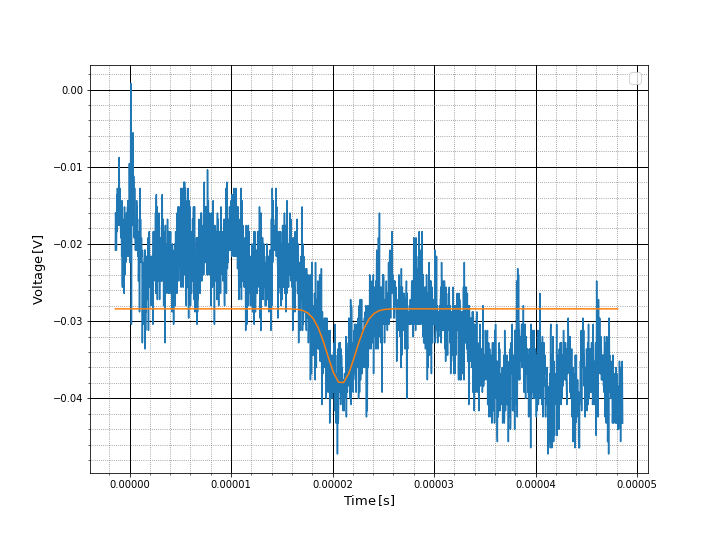
\includegraphics[scale=0.5]{Bild/S1}
	\centering
	\caption[Gaußfit an Messung bei Konst. Spannung 1]{Gaußfit an die Messungen der Elektronenwolken bei einer Spannung von $48\,$V und einem Abstand zwischen Nadel und Lase von $10.6$\,mm.}
\end{figure}
\begin{figure}
	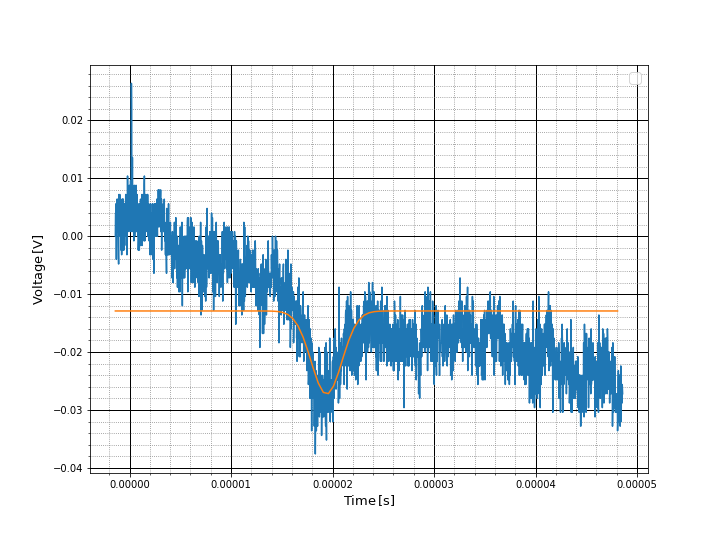
\includegraphics[scale=0.5]{Bild/S2}
	\centering
	\caption[Gaußfit an Messung bei Konst. Spannung 2]{Gaußfit an die Messungen der Elektronenwolken bei einer Spannung von $48\,$V und einem Abstand zwischen Nadel und Lase von $9.6$\,mm.}
\end{figure}
\begin{figure}
	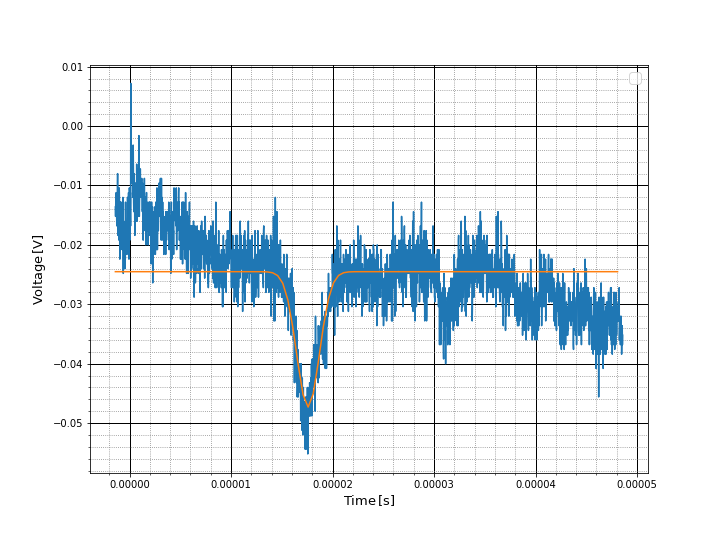
\includegraphics[scale=0.5]{Bild/S3}
	\centering
	\caption[Gaußfit an Messung bei Konst. Spannung 3]{Gaußfit an die Messungen der Elektronenwolken bei  einer Spannung von $48\,$V und einem Abstand zwischen Nadel und Lase von $8.6$\,mm.}
\end{figure}
\begin{figure}
	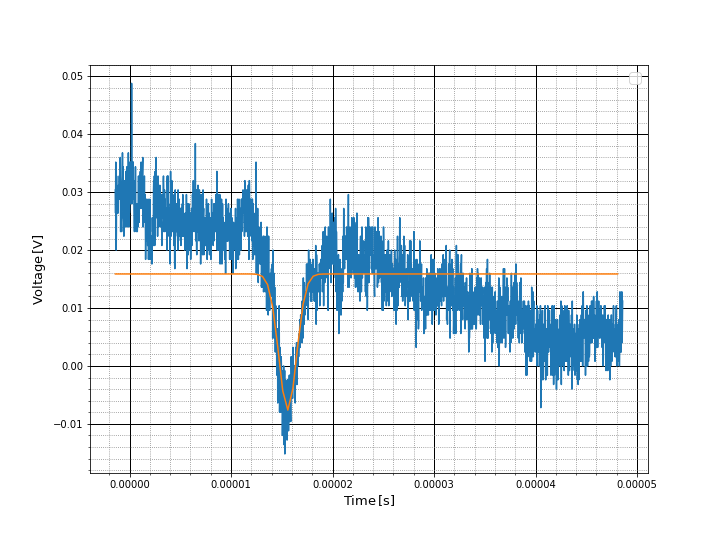
\includegraphics[scale=0.5]{Bild/S4}
	\centering
	\caption[Gaußfit an Messung bei Konst. Spannung 4]{Gaußfit an die Messungen der Elektronenwolken bei  einer Spannung von $48\,$V und einem Abstand zwischen Nadel und Lase von $7.6$\,mm.}
\end{figure}
\begin{figure}
	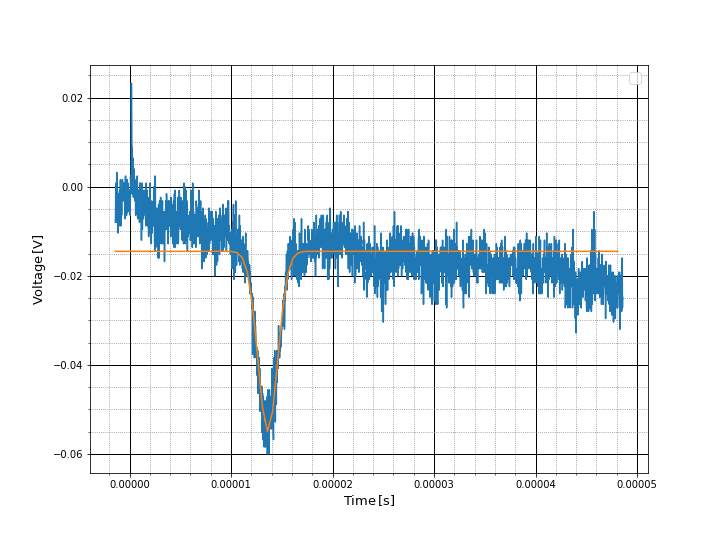
\includegraphics[scale=0.5]{Bild/S5}
	\centering
	\caption[Gaußfit an Messung bei Konst. Spannung 5]{Gaußfit an die Messungen der Elektronenwolken bei einer Spannung von $48\,$V und einem Abstand zwischen Nadel und Lase von $6.6$\,mm.}
\end{figure}
\begin{figure}
	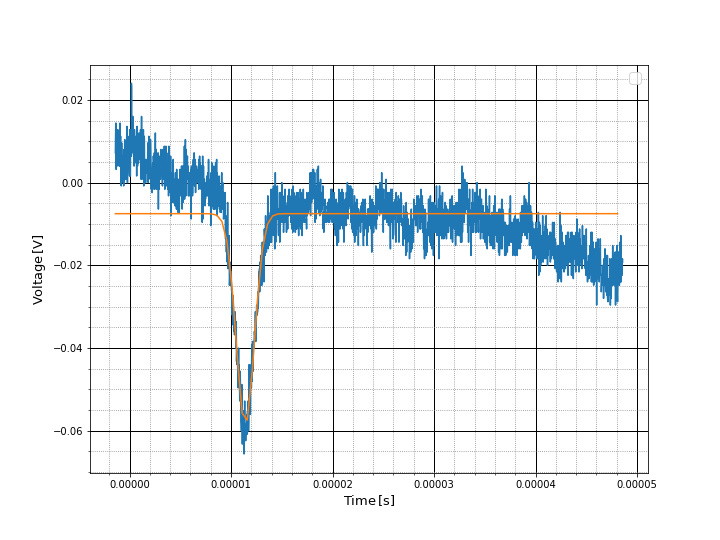
\includegraphics[scale=0.5]{Bild/S6}
	\centering
	\caption[Gaußfit an Messung bei Konst. Spannung 6]{Gaußfit an die Messungen der Elektronenwolken bei einer Spannung von $48\,$V und einem Abstand zwischen Nadel und Lase von $5.6$\,mm.}
\end{figure}
\begin{figure}
	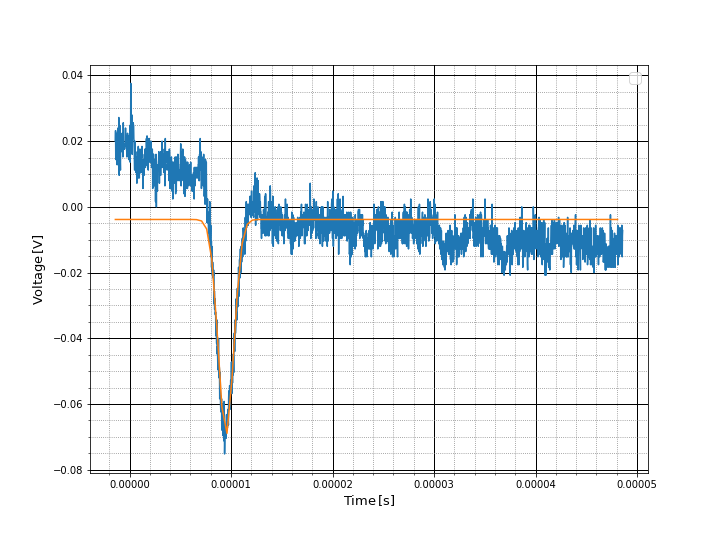
\includegraphics[scale=0.5]{Bild/S7}
	\centering
	\caption[Gaußfit an Messung bei Konst. Spannung 7]{Gaußfit an die Messungen der Elektronenwolken bei einer Spannung von $48\,$V und einem Abstand zwischen Nadel und Lase von $4.6$\,mm.}
\end{figure}
\begin{figure}
	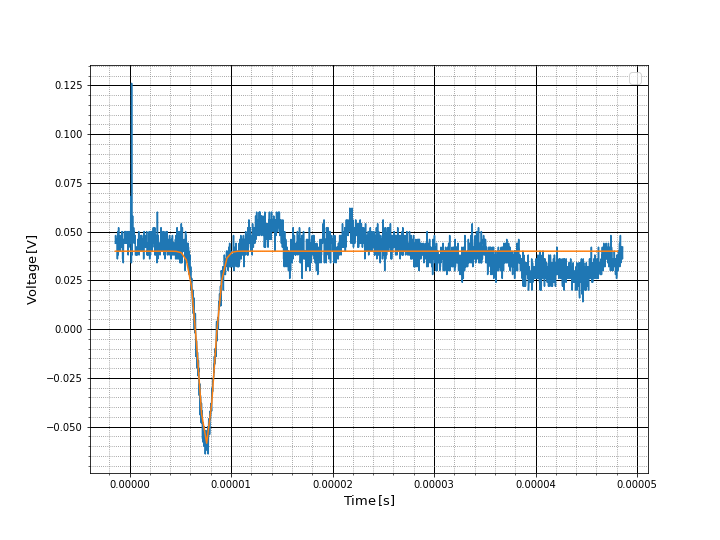
\includegraphics[scale=0.5]{Bild/S8}
	\centering
	\caption[Gaußfit an Messung bei Konst. Spannung 8]{Gaußfit an die Messungen der Elektronenwolken bei einer Spannung von $48\,$V und einem Abstand zwischen Nadel und Lase von $3.6$\,mm.}
\end{figure}

%Andere Messreihe

\begin{figure}
	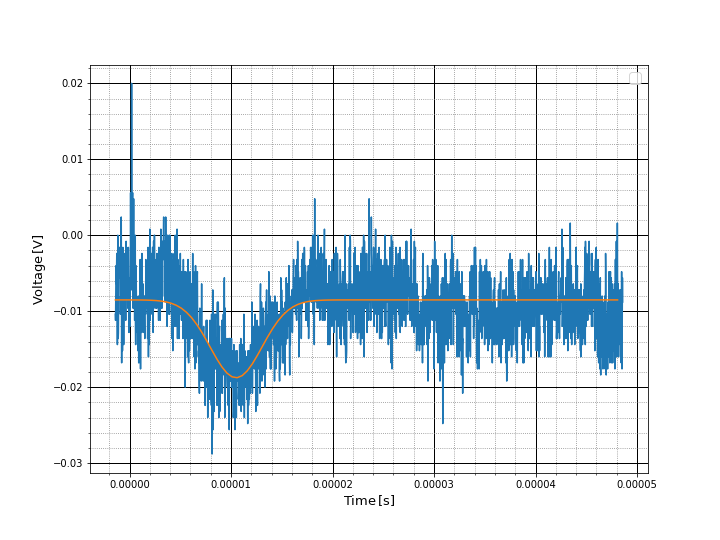
\includegraphics[scale=0.5]{Bild/A1}
	\centering
	\caption[Gaußfit an Messung bei Konst. Abstand]{Gaußfit an die Messungen der Elektronenwolken bei Konstantem Abstand von $3.6$\,mm und einer Spannung von $-13.2$\,V}
\end{figure}
\begin{figure}
	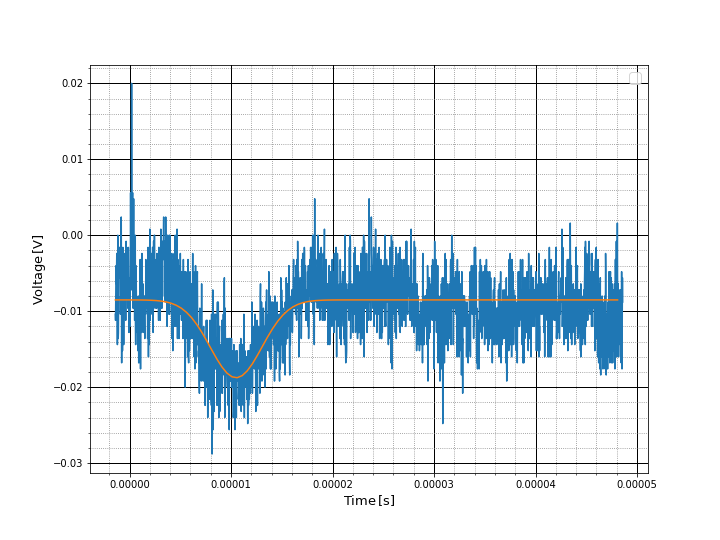
\includegraphics[scale=0.5]{Bild/A1}
	\centering
	\caption[Gaußfit an Messung bei Konst. Abstand]{Gaußfit an die Messungen der Elektronenwolken bei Konstantem Abstand von $3.6$\,mm und einer Spannung von $-15.2$\,V}
\end{figure}
\begin{figure}
	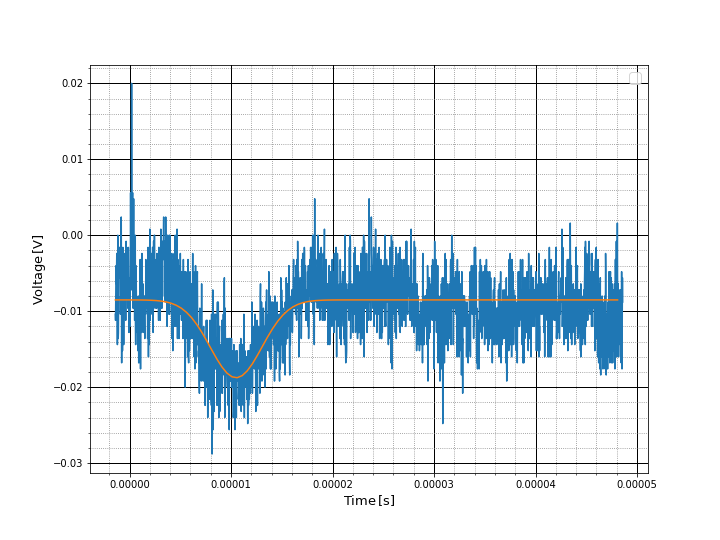
\includegraphics[scale=0.5]{Bild/A1}
	\centering
	\caption[Gaußfit an Messung bei Konst. Abstand]{Gaußfit an die Messungen der Elektronenwolken bei Konstantem Abstand von $3.6$\,mm und einer Spannung von $-18.4$\,V}
\end{figure}
\begin{figure}
	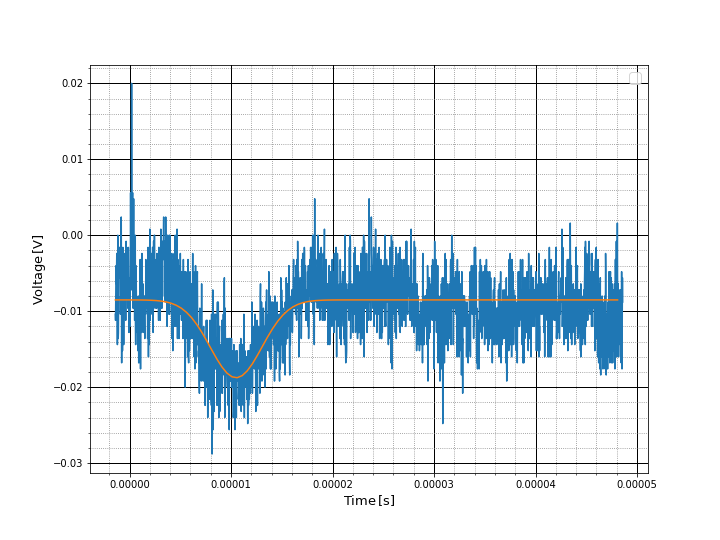
\includegraphics[scale=0.5]{Bild/A1}
	\centering
	\caption[Gaußfit an Messung bei Konst. Abstand]{Gaußfit an die Messungen der Elektronenwolken bei Konstantem Abstand von $3.6$\,mm und einer Spannung von $-20.4$\,V}
\end{figure}
\begin{figure}
	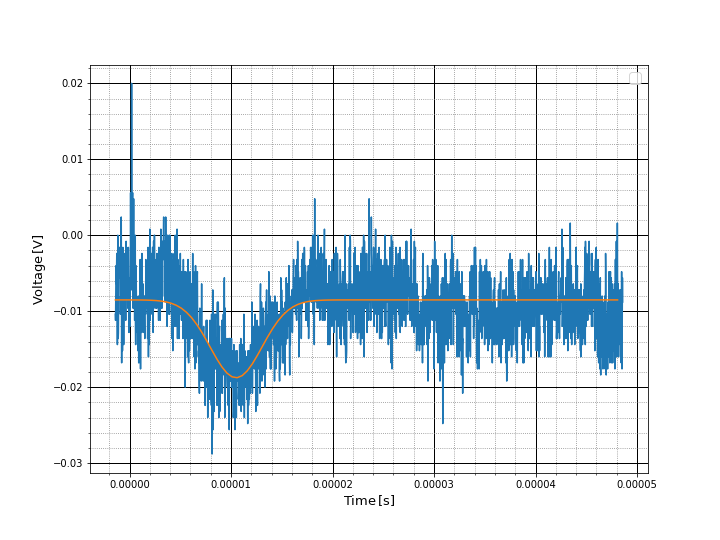
\includegraphics[scale=0.5]{Bild/A1}
	\centering
	\caption[Gaußfit an Messung bei Konst. Abstand]{Gaußfit an die Messungen der Elektronenwolken bei Konstantem Abstand von $3.6$\,mm und einer Spannung von $-22.4$\,V}
\end{figure}
\begin{figure}
	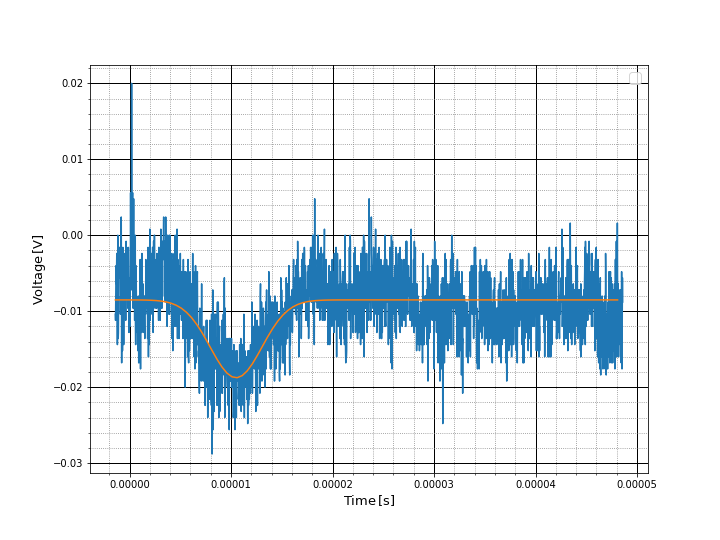
\includegraphics[scale=0.5]{Bild/A1}
	\centering
	\caption[Gaußfit an Messung bei Konst. Abstand]{Gaußfit an die Messungen der Elektronenwolken bei Konstantem Abstand von $3.6$\,mm und einer Spannung von $-24.4$\,V}
\end{figure}
\begin{figure}
	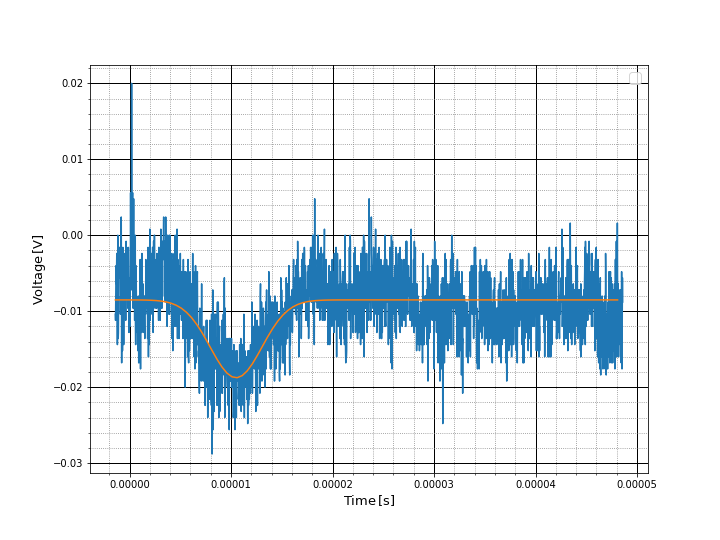
\includegraphics[scale=0.5]{Bild/A1}
	\centering
	\caption[Gaußfit an Messung bei Konst. Abstand]{Gaußfit an die Messungen der Elektronenwolken bei Konstantem Abstand von $3.6$\,mm und einer Spannung von $-28.0$\,V}
\end{figure}
\begin{figure}
	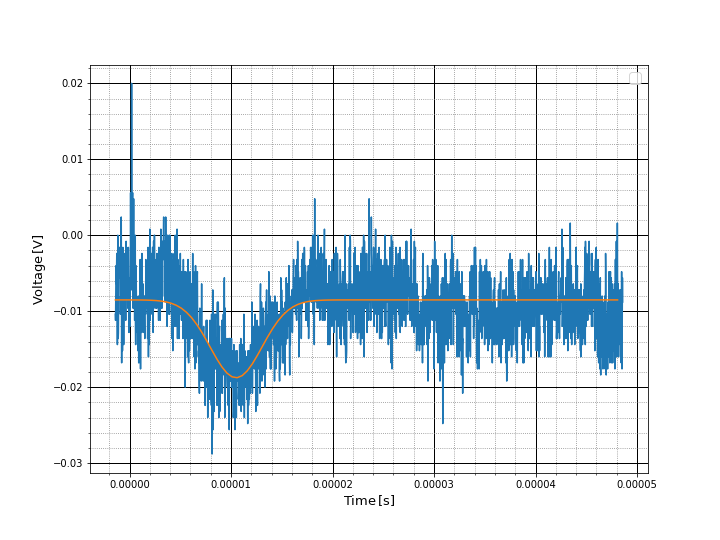
\includegraphics[scale=0.5]{Bild/A1}
	\centering
	\caption[Gaußfit an Messung bei Konst. Abstand]{Gaußfit an die Messungen der Elektronenwolken bei Konstantem Abstand von $3.6$\,mm und einer Spannung von $-32.0$\,V}
\end{figure}
\begin{figure}
	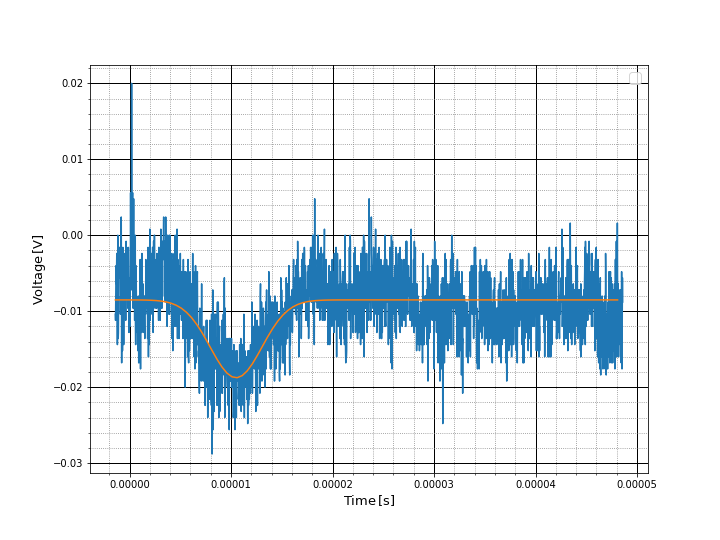
\includegraphics[scale=0.5]{Bild/A1}
	\centering
	\caption[Gaußfit an Messung bei Konst. Abstand]{Gaußfit an die Messungen der Elektronenwolken bei Konstantem Abstand von $3.6$\,mm und einer Spannung von $-36.0$\,V}
\end{figure}
\begin{figure}
	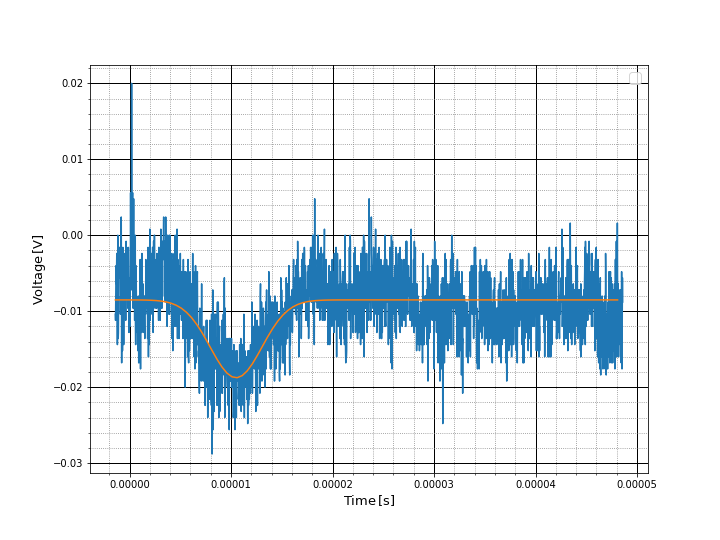
\includegraphics[scale=0.5]{Bild/A1}
	\centering
	\caption[Gaußfit an Messung bei Konst. Abstand]{Gaußfit an die Messungen der Elektronenwolken bei Konstantem Abstand von $3.6$\,mm und einer Spannung von $-40.0$\,V}
\end{figure}
\begin{figure}
	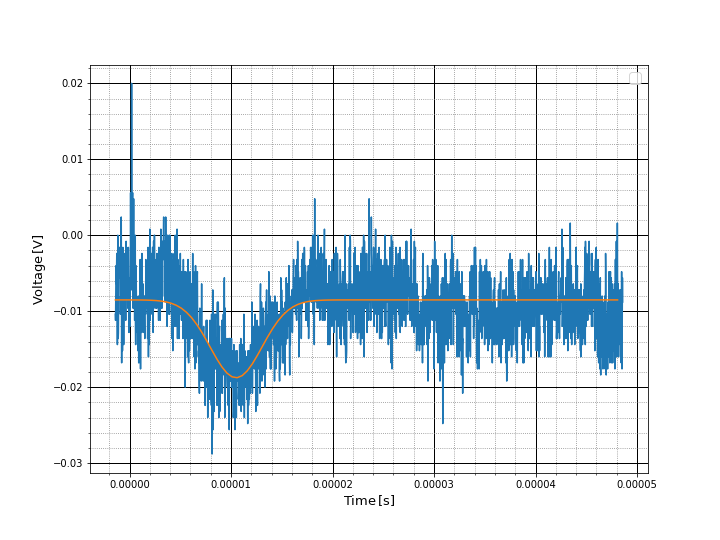
\includegraphics[scale=0.5]{Bild/A1}
	\centering
	\caption[Gaußfit an Messung bei Konst. Abstand]{Gaußfit an die Messungen der Elektronenwolken bei Konstantem Abstand von $3.6$\,mm und einer Spannung von $-44.0$\,V}
\end{figure}
\begin{figure}
	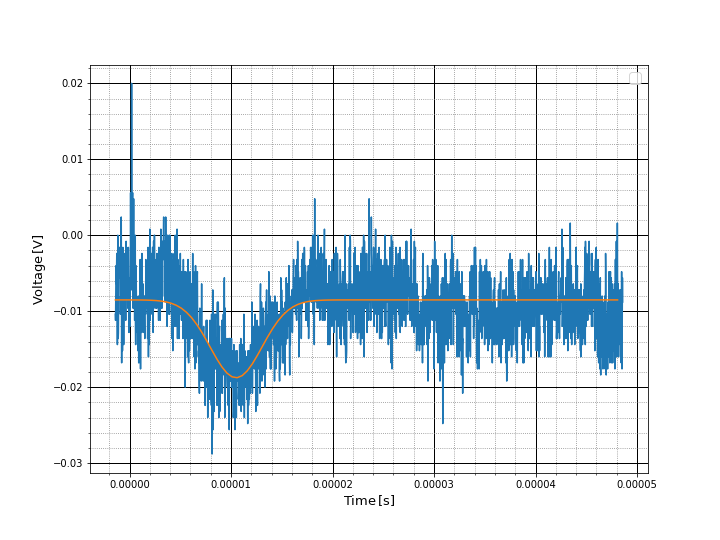
\includegraphics[scale=0.5]{Bild/A1}
	\centering
	\caption[Gaußfit an Messung bei Konst. Abstand]{Gaußfit an die Messungen der Elektronenwolken bei Konstantem Abstand von $3.6$\,mm und einer Spannung von $-46.0$\,V}
\end{figure}
\begin{figure}
	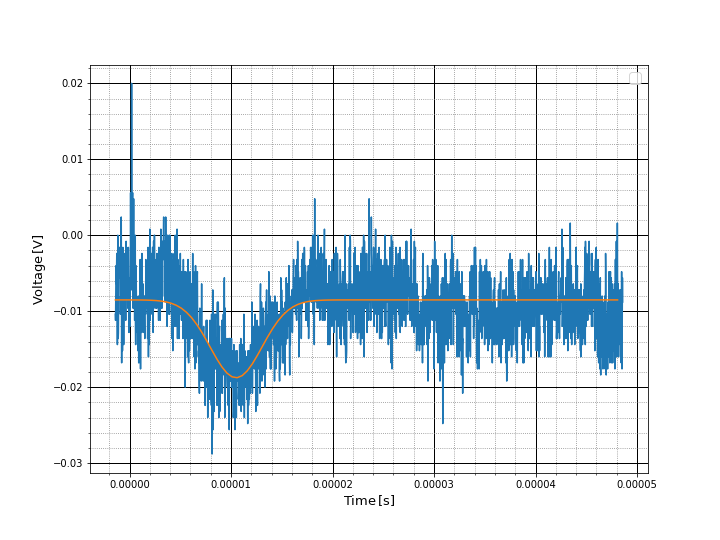
\includegraphics[scale=0.5]{Bild/A1}
	\centering
	\caption[Gaußfit an Messung bei Konst. Abstand]{Gaußfit an die Messungen der Elektronenwolken bei Konstantem Abstand von $3.6$\,mm und einer Spannung von $-48.0$\,V}
\end{figure}

%Lange Messungen

\begin{figure}[ht]
	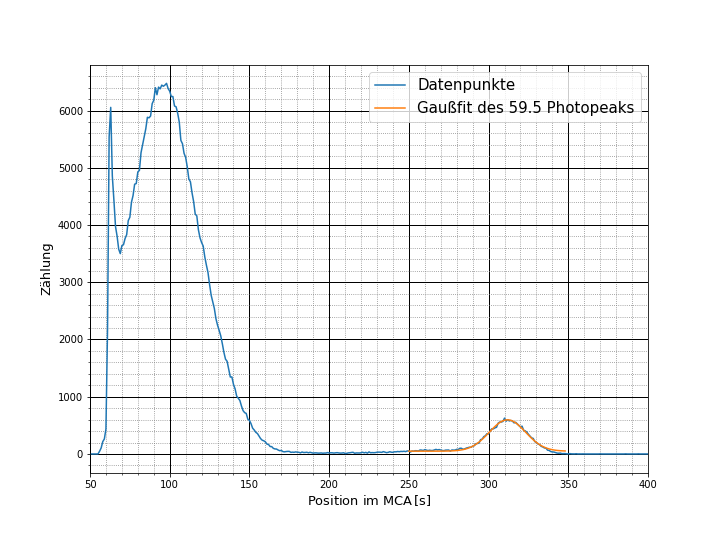
\includegraphics[scale=0.5]{Bild/ASg}
	\centering
	\caption{Gesamtes Spektrum von Americium mit Silizium aufgenommen.}
\end{figure}
\begin{figure}[ht]
	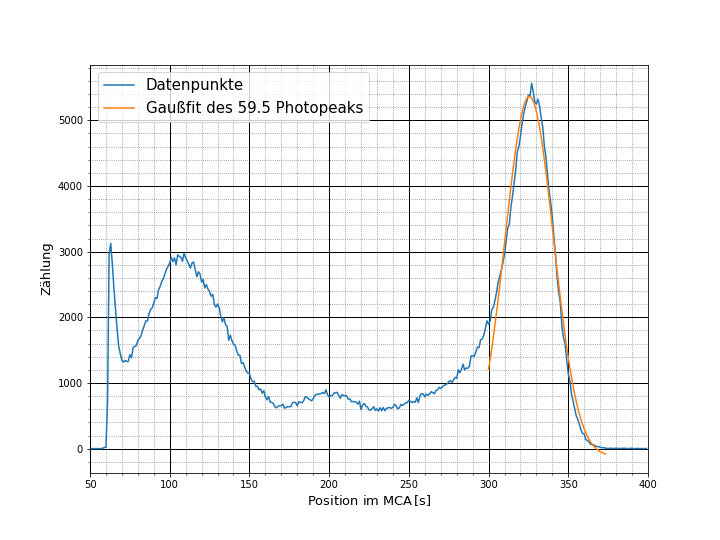
\includegraphics[scale=0.5]{Bild/ACg}
	\centering
	\caption{Gesamtes Spektrum von Americium mit CdTe aufgenommen.}
\end{figure}
\begin{figure}[ht]
	\includegraphics[scale=0.5]{Bild/CSg}
	\centering
	\caption{Gesamtes Spektrum von Cobalt mit Silizium aufgenommen.}
\end{figure}
\begin{figure}[ht]
	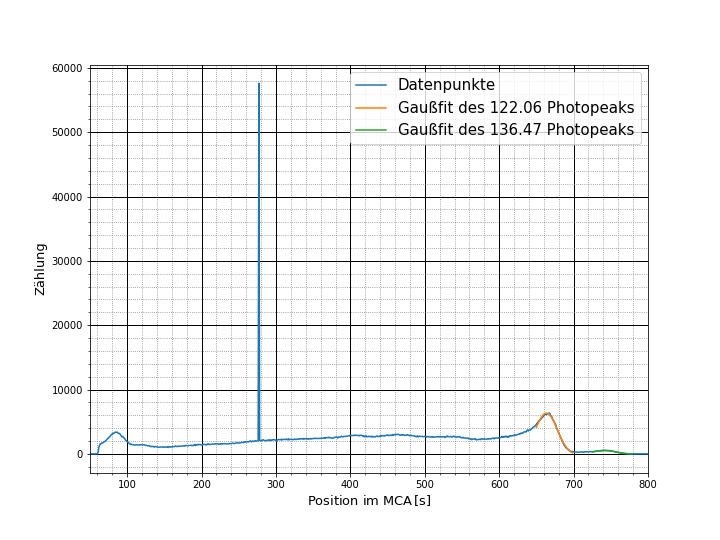
\includegraphics[scale=0.5]{Bild/CCg}
	\centering
	\caption{Gesamtes Spektrum von Cobalt mit CdTe aufgenommen.}
\end{figure}
\FloatBarrier
\subsection{Laborbuch}
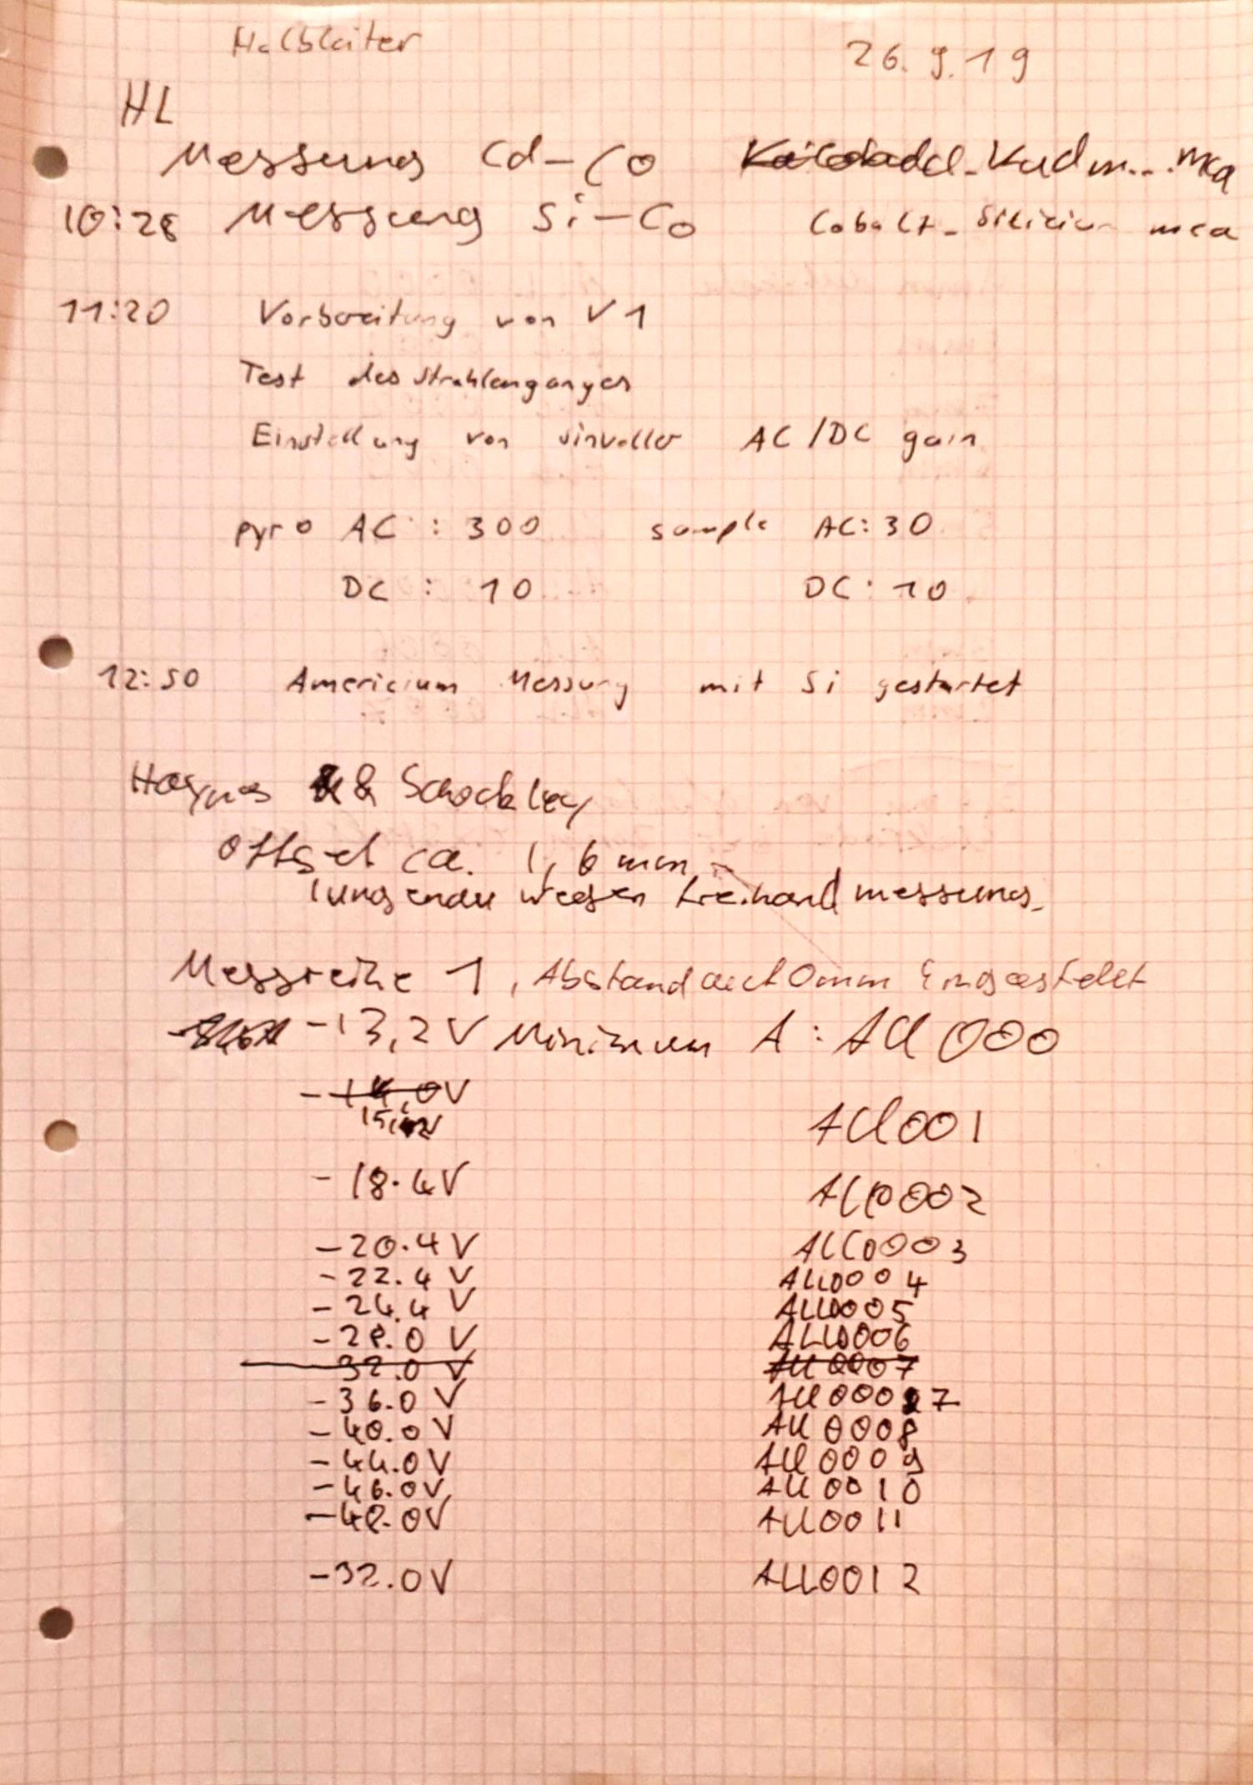
\includepdf[pages=-,scale=0.8]{Bilder/anhang/Halbleiter.pdf}